\chapter{Mengenal Python dan Anaconda}
Tujuan pembelajaran pada pertemuan pertama antara lain:
\begin{enumerate}
\item
Mengerti sejarah python, perkembangan dan penggunaan python di perusahaan
\item
Memahami tahapan instalasi python dan anaconda
\item
Memahami cara penggunaan spyder
\end{enumerate}
Tugas dengan cara dikumpulkan dengan pull request ke github dengan menggunakan format latex pada repo yang dibuat oleh asisten IRC.

\section{Teori}
Praktek teori penunjang yang dikerjakan :
\begin{enumerate}
\item
Buat Resume Sejarah Python, perbedaan python 2 dan 3, dengan bahasa yang mudah dipahami dan dimengerti. Buatan sendiri bebas plagiat(10)
\item
Buat Resume Implementasi dan penggunaan Python di perusahaan dunia, bahasa yang mudah dipahami(10)
\end{enumerate}

\section{Instalasi}
Melakukan instalasi python dan anaconda versi 3 serta uji coba spyder. Dengan menggunakan bahasa yang mudah dimengerti dan bebas plagiat. 
Dan wajib skrinsut dari komputer sendiri.
\begin{enumerate}
\item
Instalasi python 3 (5)
\item
instalasi pip(5)
\item
cara setting environment (5)
\item
mencoba entrepreter/cli melakui terminal atau cmd windows(5)
\item 
Menjalankan dan mengupdate anaconda dan spyder(5)
\item
Cara menjalankan Script hello word di spyder(5)
\item
Cara menjalankan Script otomatis login aplikasi akademik dengan library selenium dan inputan user(5)
\item
Cara pemakaian variable explorer di spyder(5)
\end{enumerate}


\section{Identasi}
Membuat file main.py dan mengisinya dengan script contoh python penggunaan selenium(minimal 20 baris) yang melibatkan inputan user, kemudian mencoba untuk mengatasi error identasi.
\begin{enumerate}
	\item
Penjelasan Identasi (10)
	\item
jenis jenis error identasi yang didapat(10)
\item
cara membaca error(10)
\item 
cara menangani errornya(10)
\end{enumerate}

\section{Presentasi Tugas}
Pada pertemuan ini, diadakan tiga penilaiain yaitu penilaian untuk tugas mingguan dengan nilai maksimal 100. Kemudian dalam satu minggu kedepan maksimal sebelum waktu mata kuliah. Ada presentasi kematerian dengan nilai presentasi yang terpisah masing-masing 100. Dan nilai terpisah untuk tutorial dari jawaban tugas di YouTube.Jadi ada tiga komponen penilaiain pada pertemuan ini yaitu :
\begin{enumerate}
	\item tugas minggu hari ini dan besok (maks 100). pada chapter ini
	\item presentasi csv (maks 100). Mempraktekkan kode python dan menjelaskan cara kerjanya.
	\item pembuatan video tutorial youtube tentang tutorial dari jawaban tugas.(nilai maks 100)
\end{enumerate}
Waktu presentasi pada jam kerja di IRC. Kriteria penilaian presentasi sangat sederhana, presenter akan ditanyai 20(10 pertanyaan program, 10 pertanyaan teori) pertanyaan tentang pemahamannya menggunakan python dan program agan dibuat error hingga presenter bisa menyelesaikan errornya. jika presenter tidak bisa menjawab satu pertanyaan asisten maka nilai nol. Jika semua pertanyaan bisa dijawab maka nilai 100. Presentasi bisa diulang apabila gagal, sampai bisa mendapatkan nilai 100 dalam waktu satu minggu kedepan.
\section{Jawaban}
\subsection{Teori}
\begin{enumerate}
    \item-Sejarah Python
    
    Pada tahun 1990 Python dikembangkan oleh Guido van Rossum  di Stichting Mathematisch Centrum (CWI), Amsterdam sebagai kelanjutan dari bahasa pemrograman ABC.Guido pindah ke CNRI di Virginia Amerika pada tahun 1995 sambil tetap melakukan pengembangan Python.Guido dan para pengembang inti Python pindah ke BeOpen.com yang merupakan sebuah perusahaan komersial dan membentuk BeOpen PythonLabs. Python 2.0 dipublish oleh BeOpen. Setelah mempublish Python 2.0, Guido dan beberapa anggota tim PythonLabs pindah ke DigitalCreations.

Saat ini pengembangan Python masih terus dilakukan oleh sekumpulwn pemrogram yang dipimpin oleh Guido dan Python Software Foundation. Python Software Foundation adalah sebuah organisasi non-profit yang dibentuk sebagai pemegang hak cipta intelektual Python sejak versi 2.1 dan dengan demikian mencegah Python dimiliki oleh perusahaan komersial. Saat ini distribusi Python sudah mencapai versi 2.7.14 dan versi 3.6.3

Nama Python sendiri dipilih oleh Guido sebagai nama bahasa ciptaannya karena Guido menyukai acara televisi bernama Monty Python's Flying Circus. Oleh karena itu seringkali ungkapan-ungkapan khas dari acara tersebut seringkali muncul dalam korespondensi antar pengguna Python.

-Perbedaan Python 2 dan 3 

Python 2 dalam menggunakan syntax print bisa menggunakan tanda kurung maupun tidak, sedangkan di Python 3 syntax print harus menggunakan kurung.

Pada Python 2, semua tipe data angka yang tidak mengandung desimal akan dianggap sebagai integer.Pada Python 3, pembagian pada bilangan integer lebih intuitif.

Ketika bahasa pemrograman menangani tipe data string, mereka bisa melakukan beberapa cara berbeda sehingga komputer dapat mengubah angka ke huruf dan simbol lain.Python 2 menggunakan alfabet ASCII secara default, sehingga ketika kita mengetik “Halo!”  maka Python 2 menangani string sebagai ASCII.

Untuk menggunakan unicode yang lebi,kita harus mengetik u”Halo!” , dengan tambahan u  di depannya yang berarti Unicode.

Python 3 menggunakan Unicode secara default,untuk mempermudah programmer, lebih hemat waktu dan mudah untuk diisikan dan ditampilkan. Karena Unicode mendukung berbagai karakter linguistik yang beragam termasuk menampilkan emoji, penggunaan karakter secara default dengan encoding memastikan perangkat mobile didukung oleh program yang kita buat.

Jika kita ingin kode Python 3 kita mendukung Python 2, tambahkan u di depan string.


\item
Python banyak dimanfaatkan di ranah analisis data oleh banyak perusahaan besar, contohnya Spotify dan Netflix.Python juga banyak digunakan untuk pengembangan Artificial Intelligence atau AI, dan Python bisa juga digunakan untuk membuat special effect pada film-film Hollywood.
\end{enumerate}
\subsection{Instalasi}
\begin{enumerate}
    \item Instalasi python
    
   -  Pertama bukan instalan Python nya,pilih customize installation untuk memilih direktori instalasi.
    
    \begin{center}
       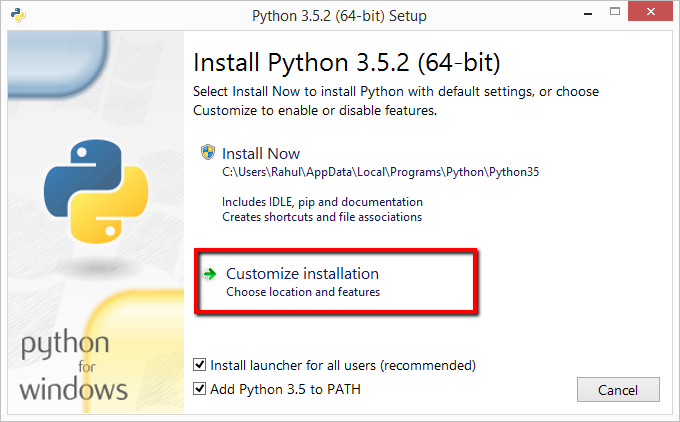
\includegraphics[width=10cm]{section/install-python-1.png}
    \ 
    \end{center}
 
- Lalu Centang semua jika dibutuhkan.


    \begin{center}
        
    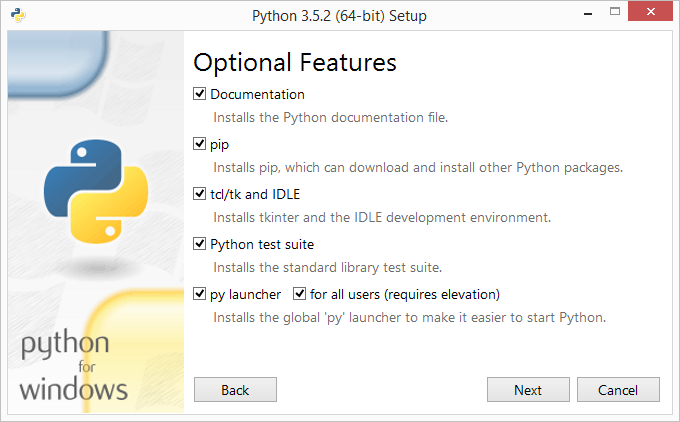
\includegraphics[width=10cm]{section/install-python-3.png}
    \end{center}
    - Pilih direktori instalasi jika di butuhkan atau boleh langsung klik install.
    
    \begin{center}
        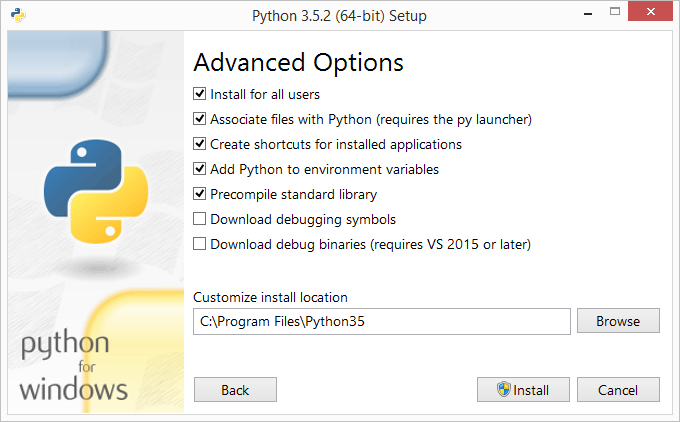
\includegraphics[width=10cm]{section/install-python-4.png}
    \end{center}
    
    - Akan muncul pesan successful, klik close dan python akan menyelesaikan instalasinya.
     
     \begin{center}
         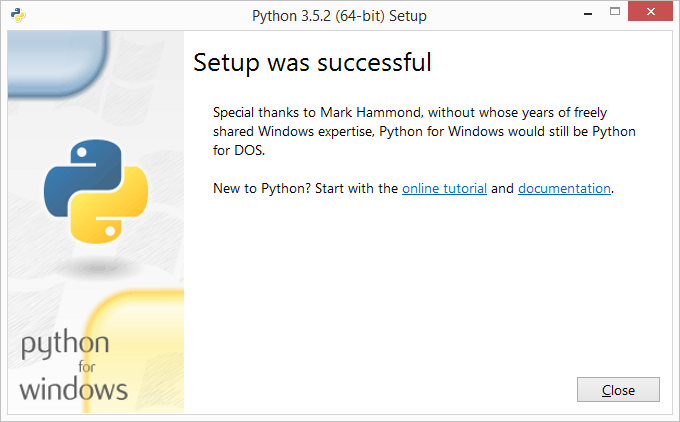
\includegraphics[width=10cm]{section/install-python-5.png}
     \end{center}
    

    
 \item instalasi pip
 
  Download pip terlebih dahulu di website resminnya lalu klik file yg telah di download, tapi untuk python versi 2.7.9 keatas dan python versi 3.4 keatas pip akan terinstall secara default.
  \begin{center}
     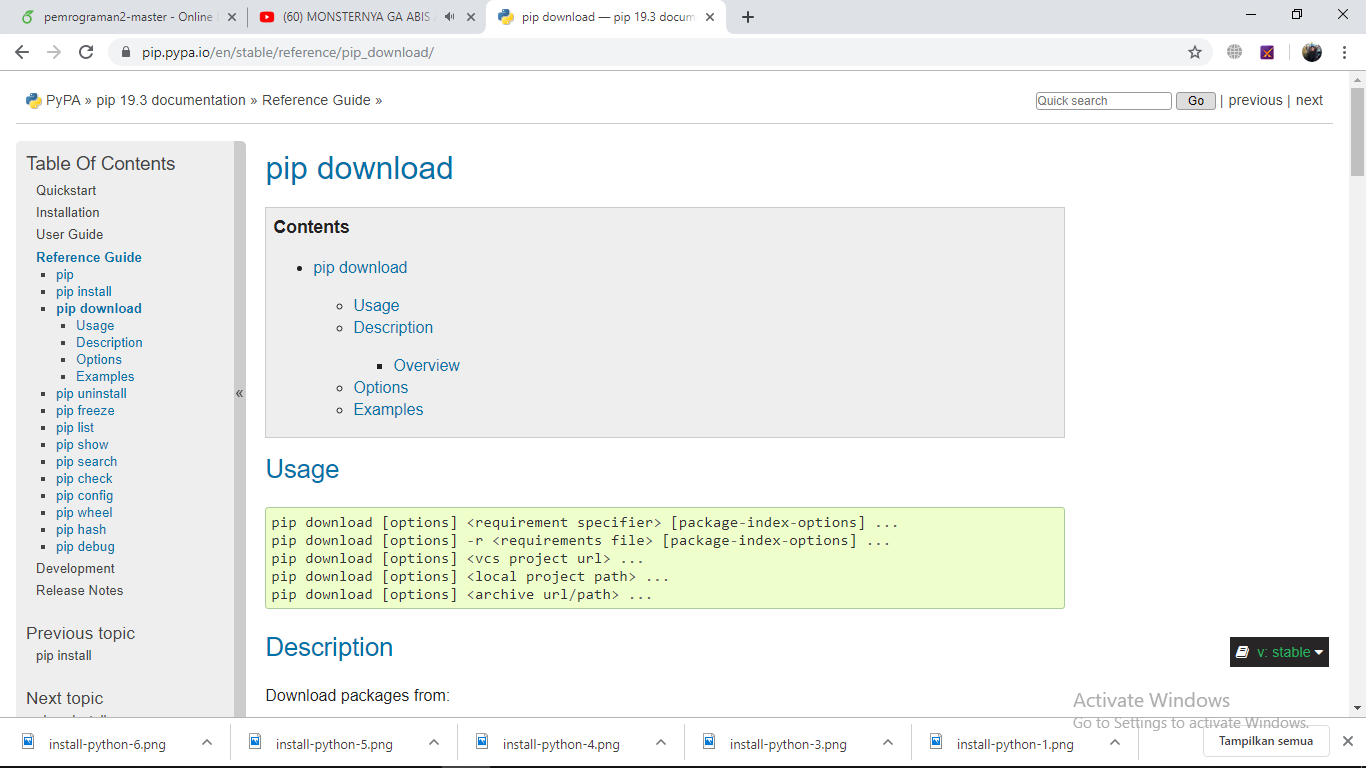
\includegraphics[width=10cm]{section/Screenshot (1).png} 
  \end{center}
  \item Cara setting environment
  
  - Masuk ke system pada Control Panel
Control Panel\ System and Security\ System
 Kemudian klik   “Advanced system settings“
  \begin{center}
      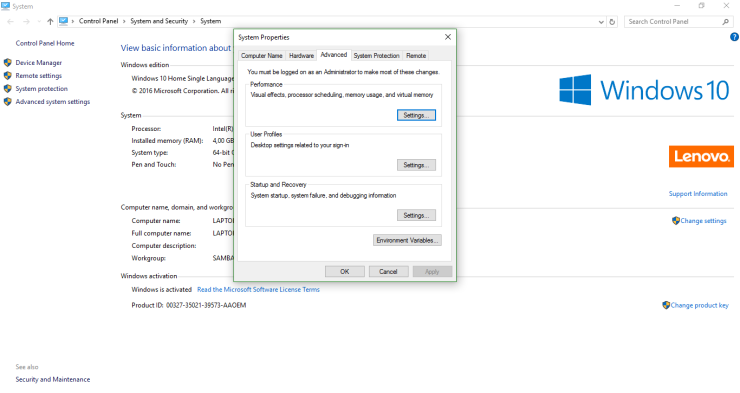
\includegraphics[width=10cm]{section/capture006.png}
  \end{center}
  -Lalu klik “Environment Variables” maka akan muncul pop up “Environment Variables”
Pada bagian System variables, scroll sampai ketemu Path.
\begin{center}
    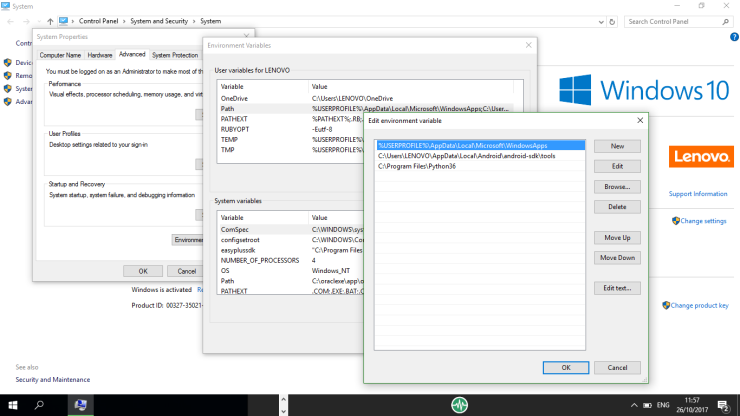
\includegraphics[width=10cm]{section/capture007.png}
\end{center}
    -Seleksi/klik Path dan kemudian klik Edit
Maka akan muncul pop up “Edit System variable”
,buka notepad copas semua Variable value.
Pada bagian paling kanan/ujung “Variable value”
tambahkan path  “;C:\Python36\”  tanpa tanda petik
dan klik OK pada jendela Edit System variable.
klik OK pada jendela Environment Variables.
klik OK pada jendela System Properties.
dan close Control Panel,kalau sudah selesai akan muncul seperti ini.
\begin{center}
    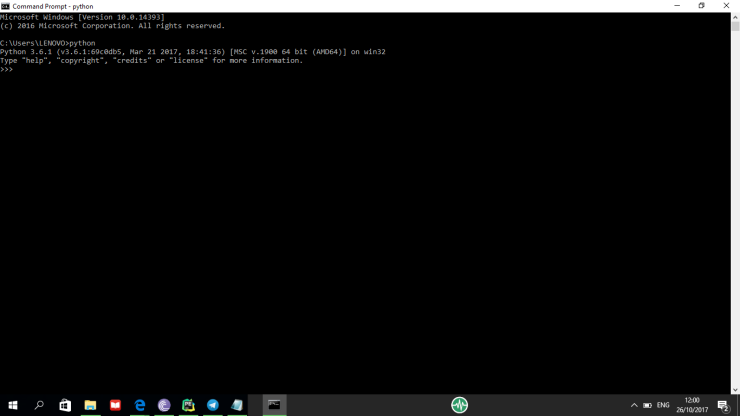
\includegraphics[width=10cm]{section/capture008.png}
\end{center}
\item Enterpreter/cli melalui terminal atau cmd windows

-interpreter cmd
\begin{center}
    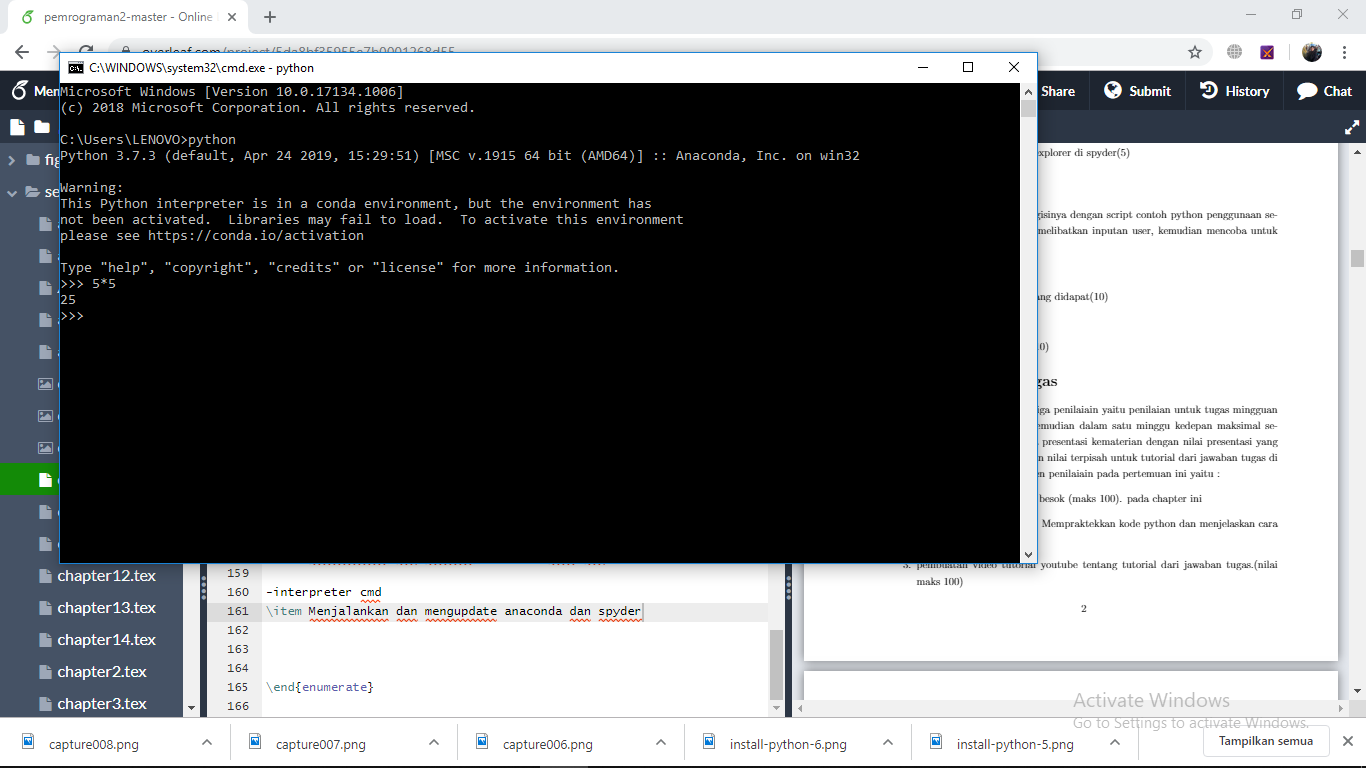
\includegraphics[width=10cm]{section/Screenshot (2).png}
\end{center}
\item Menjalankan dan mengupdate anaconda dan spyder
\begin{center}
    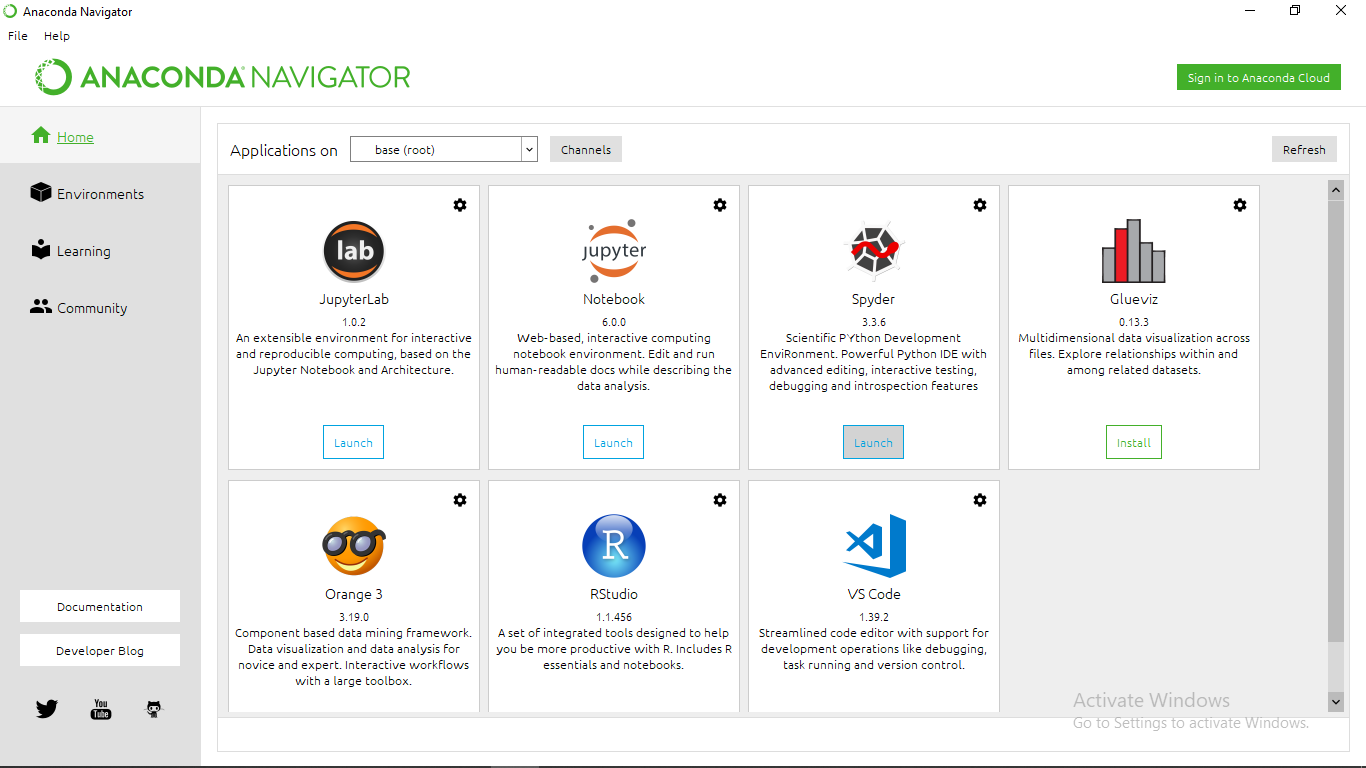
\includegraphics[width=10cm]{section/Screenshot (3).png}
    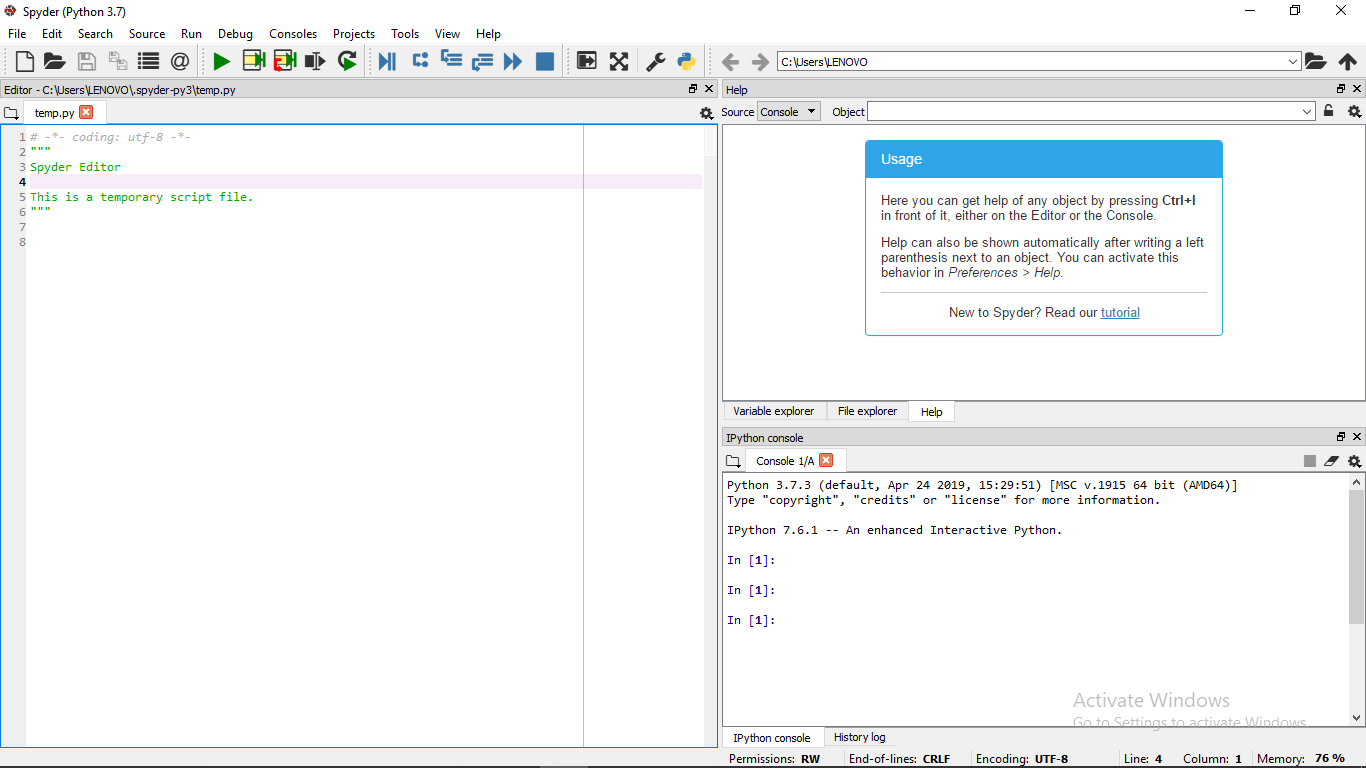
\includegraphics[width=10cm]{section/Screenshot (4).png}
\end{center}
\item Menjalankan Script hello world di spyder
\begin{center}
    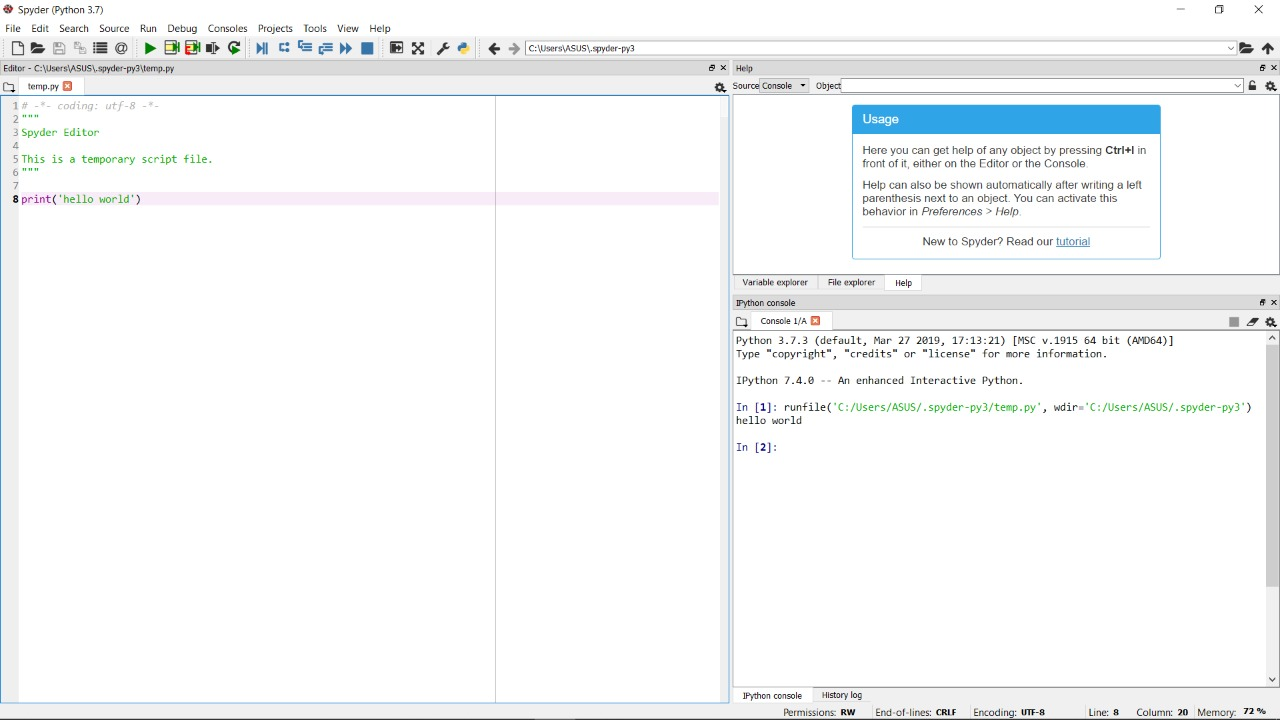
\includegraphics[width=10cm]{section/hello world.jpg}
\end{center}
\item Cara menjalankan script otomatis login aplikasi akademik dengan library selenium dan inputan user
\item Cara pemakaian variable di explorer di spyder
\begin{center}
    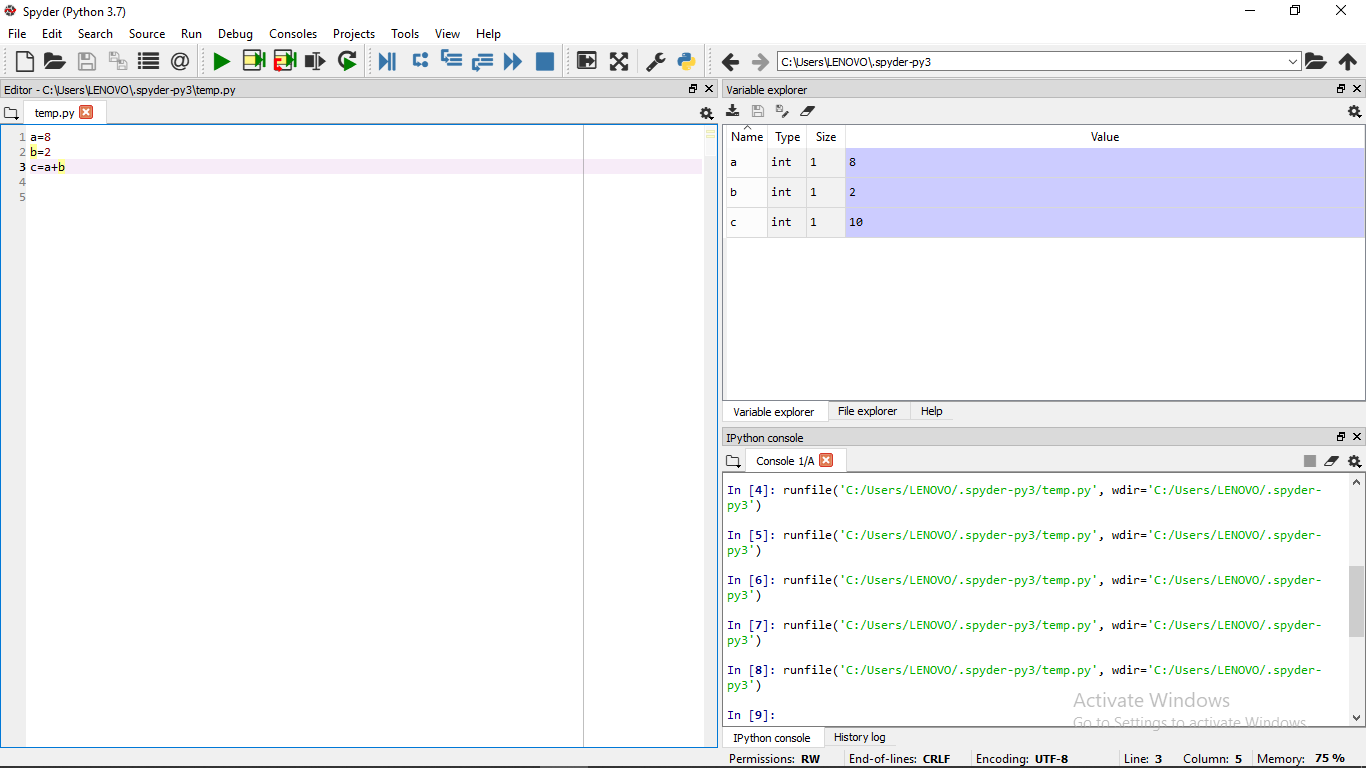
\includegraphics[width=10cm]{section/Screenshot (5).png}
\end{center}

    
    
\end{enumerate}
